% RAISE Doctoral Networks for AI in Science -- Beamer Slide Deck
% Data: v3-corrected figures from MSCA Work Programme 2026-2027
% Compiled with: pdflatex
\documentclass[aspectratio=169]{beamer}

%%% ---------------------------------------------------------------
%%% PACKAGES
%%% ---------------------------------------------------------------
\usepackage[T1]{fontenc}
\usepackage{lmodern}
\usepackage{tikz}
\usetikzlibrary{shapes,arrows.meta,positioning,calc,decorations.pathreplacing}
\usepackage{booktabs}
\usepackage{colortbl}
\usepackage{hyperref}
\usepackage{array}

%%% ---------------------------------------------------------------
%%% COLOURS
%%% ---------------------------------------------------------------
\definecolor{euBlue}{HTML}{003399}
\definecolor{euGold}{HTML}{FFCC00}
\definecolor{euLightBlue}{HTML}{D6E4F0}
\definecolor{euDarkGold}{HTML}{CC9900}
\definecolor{euGreen}{HTML}{009933}
\definecolor{euRed}{HTML}{CC3333}

%%% ---------------------------------------------------------------
%%% BEAMER THEME CONFIGURATION
%%% ---------------------------------------------------------------
\usetheme{default}
\usecolortheme{default}

% Title bar
\setbeamercolor{frametitle}{bg=euBlue,fg=white}
\setbeamercolor{title}{fg=euBlue}
\setbeamercolor{subtitle}{fg=euBlue!70!black}
\setbeamercolor{structure}{fg=euBlue}

% Bullet styling
\setbeamercolor{itemize item}{fg=euBlue}
\setbeamercolor{itemize subitem}{fg=euBlue!70}
\setbeamertemplate{itemize item}{\raisebox{0.15ex}{\small$\blacktriangleright$}}
\setbeamertemplate{itemize subitem}{\raisebox{0.1ex}{\scriptsize$\bullet$}}

% Block colours
\setbeamercolor{block title}{bg=euBlue,fg=white}
\setbeamercolor{block body}{bg=euLightBlue,fg=black}
\setbeamercolor{block title alerted}{bg=euRed,fg=white}
\setbeamercolor{block body alerted}{bg=euRed!10,fg=black}
\setbeamercolor{block title example}{bg=euGreen,fg=white}
\setbeamercolor{block body example}{bg=euGreen!10,fg=black}

% Footer with frame numbering
\setbeamertemplate{navigation symbols}{}
\setbeamertemplate{footline}{%
  \hfill%
  \usebeamercolor[fg]{structure}%
  \scriptsize\insertframenumber\,/\,\inserttotalframenumber%
  \hspace*{4pt}\vspace{2pt}%
}

% Reduce frametitle padding
\setbeamertemplate{frametitle}{%
  \vspace*{2pt}%
  \insertframetitle%
  \vspace*{1pt}%
}

%%% ---------------------------------------------------------------
%%% CUSTOM COMMANDS
%%% ---------------------------------------------------------------
\newcommand{\eur}[1]{EUR\,#1}
\newcommand{\highlight}[1]{\textcolor{euBlue}{\textbf{#1}}}
\newcommand{\goldhl}[1]{\colorbox{euGold}{\textcolor{euBlue}{\textbf{#1}}}}

%%% ---------------------------------------------------------------
%%% TITLE PAGE DATA
%%% ---------------------------------------------------------------
\title{RAISE Doctoral Networks\\for AI in Science}
\subtitle{HORIZON-RAISE-2026-01-03\quad|\quad\eur{30 Million}\quad|\quad Deadline: 24 November 2026}
\author{Your Name Here}
\date{\today}
\institute{}

%%% ===============================================================
\begin{document}

%%% ---------------------------------------------------------------
%%% SLIDE 1 -- TITLE
%%% ---------------------------------------------------------------
\begin{frame}[plain]
\vfill
\begin{center}
  {\usebeamerfont{title}\usebeamercolor[fg]{title}\LARGE RAISE Doctoral Networks\\[6pt]for AI in Science\par}
  \vspace{10pt}
  
\begin{tikzpicture}
    \draw[euGold, line width=2pt] (0,0) -- (10,0);
  \end{tikzpicture}
  \vspace{10pt}

  {\large\textcolor{euBlue}{HORIZON-RAISE-2026-01-03}}\\[6pt]
  {\large \goldhl{\eur{30 Million}} \quad\textcolor{euBlue}{|}\quad
   \textbf{Deadline: 24 November 2026, 17:00 Brussels}}\\[14pt]
  {\normalsize\textcolor{gray}{Presenter Name $\cdot$ Institution $\cdot$ \today}}
\end{center}
\vfill
\end{frame}

%%% ---------------------------------------------------------------
%%% SLIDE 2 -- WHAT IS RAISE?
%%% ---------------------------------------------------------------
\begin{frame}{What Is RAISE?  (Brief Context)}
\begin{itemize}
  \item \highlight{RAISE} = Resource for AI in Science in Europe
  \item Virtual research institute launched November 2025
  \item EUR\,107\,M pilot under Horizon Europe
  \item Four pillars:
    \begin{itemize}
      \item Computational Power
      \item Data
      \item \textbf{Talent} $\leftarrow$ \textit{this presentation}
      \item Funding
    \end{itemize}
  \item The \highlight{Talent} pillar funds \textbf{Doctoral Networks} (DNs)
  \item This talk: everything you need to know about the RAISE DN call
\end{itemize}
\end{frame}

%%% ---------------------------------------------------------------
%%% SLIDE 3 -- CALL AT A GLANCE
%%% ---------------------------------------------------------------
\begin{frame}{The RAISE DN Call at a Glance}
\begin{block}{Key Facts}
\renewcommand{\arraystretch}{1.35}
\begin{tabular}{@{}l l@{}}
  \textbf{Call identifier}   & HORIZON-RAISE-2026-01-03 \\
  \textbf{Action type}       & TMA -- Doctoral Networks \\
  \textbf{Total budget}      & \eur{30 million} \\
  \textbf{Call opens}        & 28 May 2026 \\
  \textbf{Submission deadline} & \textbf{24 November 2026} (17:00 CET, Brussels) \\
  \textbf{Number of projects}  & Depends on proposal quality and size \\
\end{tabular}
\end{block}
\vspace{6pt}
\textcolor{euBlue}{\small Proposals are submitted via the Funding \& Tenders portal under the MSCA Doctoral Networks call.}
\end{frame}

%%% ---------------------------------------------------------------
%%% SLIDE 4 -- WHY APPLY?
%%% ---------------------------------------------------------------
\begin{frame}{Why Apply?  Strategic Advantages}
\begin{enumerate}
  \item \highlight{Second-chance mechanism} -- Strong MSCA proposals get a second funding pathway through the RAISE budget
  \item \highlight{RAISE community membership} -- Access to shared AI infrastructure, data, and a pan-European research community
  \item \highlight{Dual evaluation track} -- Your proposal can be funded via the main MSCA budget \emph{or} the RAISE budget
  \item \highlight{Cross-disciplinary openness} -- All scientific disciplines welcome, not only STEM
  \item \highlight{AI-focus premium} -- Aligns with growing EU investment in AI for science (EUR\,3\,B+ annual target)
\end{enumerate}
\end{frame}

%%% ---------------------------------------------------------------
%%% SLIDE 5 -- AI SCOPE: WHAT QUALIFIES
%%% ---------------------------------------------------------------
\begin{frame}{AI in Science Scope -- What Qualifies}
Every doctoral project in the network must meet \textbf{all} of the following:
\vspace{4pt}
\begin{enumerate}
  \item Doctoral candidates must \highlight{develop} or \highlight{significantly participate} in developing innovative AI systems, models, or tools
  \item AI must \highlight{substantially innovate} how scientific information is analysed
  \item AI development must be \highlight{integral and indispensable} to the research
  \item Scientific advancements must be \highlight{directly dependent} on the AI
  \item All candidates must receive dedicated \textbf{doctoral-level AI training}
\end{enumerate}
\vspace{6pt}
\textcolor{euBlue}{\small Key word: \emph{integral}, not merely \emph{instrumental}.}
\end{frame}

%%% ---------------------------------------------------------------
%%% SLIDE 6 -- AI SCOPE: WHAT DOES NOT QUALIFY + TikZ #1
%%% ---------------------------------------------------------------
\begin{frame}{AI Scope -- What Does NOT Qualify}
\begin{columns}[T]
\begin{column}{0.42\textwidth}
Does \textbf{not} qualify:
\begin{itemize}
  \item Pure CS/AI research published only in CS venues
  \item \textbf{Instrumental} use of existing AI tools for data processing
  \item Using general-purpose tools without innovation
\end{itemize}
\vspace{6pt}
\textcolor{euBlue}{\footnotesize \textbf{Key distinction:}\\
Developing new AI \emph{for} science \checkmark\\
Using existing AI \emph{as} a tool \texttimes}
\end{column}
\begin{column}{0.55\textwidth}
% -- TikZ Diagram 1: Integral vs Instrumental --
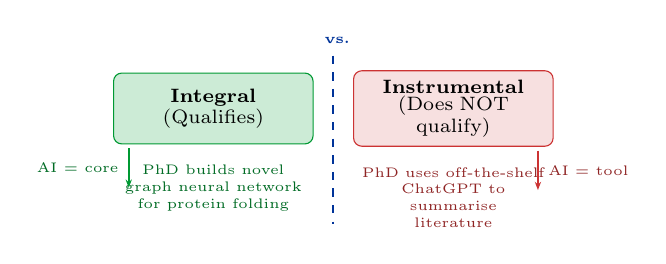
\begin{tikzpicture}[
    every node/.style={font=\scriptsize},
    box/.style={draw, rounded corners=3pt, minimum width=2.5cm,
                minimum height=0.9cm, text width=2.3cm, align=center,
                font=\tiny},
  ]
  % Left column - qualifies
  \node[box, fill=euGreen!20, draw=euGreen, text=black] (int)
    {\scriptsize\textbf{Integral}\\(Qualifies)};
  \node[below=4pt of int, text width=2.5cm, align=center, text=euGreen!70!black,
        font=\tiny]
    (intex) {PhD builds novel\\graph neural network\\for protein folding};

  % Right column - does not qualify
  \node[box, fill=euRed!15, draw=euRed, text=black, right=0.5cm of int] (ins)
    {\scriptsize\textbf{Instrumental}\\(Does NOT qualify)};
  \node[below=4pt of ins, text width=2.5cm, align=center, text=euRed!70!black,
        font=\tiny]
    (insex) {PhD uses off-the-shelf\\ChatGPT to summarise\\literature};

  % Arrows and labels
  \draw[-{Stealth[length=3pt]}, euGreen, thick]
    (int.south west) ++(0.2,-0.05) -- ++(0,-0.5)
    node[midway, left, text=euGreen!70!black, font=\tiny] {AI = core};
  \draw[-{Stealth[length=3pt]}, euRed, thick]
    (ins.south east) ++(-0.2,-0.05) -- ++(0,-0.5)
    node[midway, right, text=euRed!70!black, font=\tiny] {AI = tool};

  % Central divider
  \draw[euBlue, dashed, thick] ($(int.north east)!0.5!(ins.north west)+(0,0.2)$)
    -- ($(int.south east)!0.5!(ins.south west)+(0,-1.0)$);
  \node[above=0.25cm of int.north east, anchor=south, xshift=0.3cm,
        font=\tiny\bfseries, text=euBlue] {vs.};
\end{tikzpicture}
\end{column}
\end{columns}
\end{frame}

%%% ---------------------------------------------------------------
%%% SLIDE 7 -- THREE NETWORK TYPES
%%% ---------------------------------------------------------------
\begin{frame}{Three Network Types}
\renewcommand{\arraystretch}{1.25}
\begin{center}
\scriptsize
\begin{tabular}{@{}>{\bfseries}l >{\centering\arraybackslash}p{2.8cm}
                     >{\centering\arraybackslash}p{3.2cm}
                     >{\centering\arraybackslash}p{2.8cm}@{}}
  \toprule
  & \textbf{Standard DN} & \textbf{Industrial Doctorates} & \textbf{Joint Doctorates} \\
  \midrule
  Max duration        & 48 months & 48 months & 60 months \\
  Key feature         & Standard partnerships & Strong non-academic sector & Joint/multiple degrees \\
  \rowcolor{euLightBlue}
  Secondment rule     & Up to 50\% of fellowship & No cap (min 50\% in non-academic sector) & No cap \\
  Fellowship per DC   & 3--36 months & 3--36 months & 3--48 months \\
  Max person-months   & 540 & 540 & 540 \\
  \bottomrule
\end{tabular}
\end{center}
\vspace{4pt}
\textcolor{euBlue}{\small All three types are eligible under the RAISE DN call. Choose based on consortium structure.}
\end{frame}

%%% ---------------------------------------------------------------
%%% SLIDE 8 -- CONSORTIUM REQUIREMENTS
%%% ---------------------------------------------------------------
\begin{frame}{Consortium Requirements}
\begin{itemize}
  \item Minimum \highlight{3 independent legal entities} from \highlight{3 different} EU Member States or Associated Countries
  \item At least \textbf{1 entity must be in an EU Member State}
  \item Every beneficiary must employ \textbf{at least 1 doctoral candidate}
  \item Funding concentration cap: max \textbf{40\%} of EU contribution to same-country beneficiaries
  \item Same 40\% cap applies to international organisations
  \item Proposal length: max \textbf{30 pages} (excluding attachments)
\end{itemize}
\vspace{6pt}
\begin{alertblock}{China Exclusion}
Legal entities established in \textbf{China} are \textbf{not eligible} to participate as beneficiaries, affiliated entities, or associated partners.
\end{alertblock}
\end{frame}

%%% ---------------------------------------------------------------
%%% SLIDE 9 -- MOBILITY RULE
%%% ---------------------------------------------------------------
\begin{frame}{Eligibility -- The Mobility Rule}
\begin{block}{Core Rule}
A recruited researcher must \textbf{not} have resided or carried out their main activity in the country of the recruiting beneficiary for more than \highlight{12 months in the 36 months} immediately before the recruitment date.
\end{block}
\vspace{8pt}
\textbf{Exceptions:}
\begin{itemize}
  \item Refugees and EU temporary-protection beneficiaries are \textbf{exempt}
  \item Compulsory national service is \textbf{not counted}
  \item Short stays (conferences, holidays) are \textbf{not counted}
\end{itemize}
\vspace{6pt}
\textcolor{euBlue}{\small This rule ensures cross-border mobility -- a core MSCA principle.}
\end{frame}

%%% ---------------------------------------------------------------
%%% SLIDE 10 -- HOW TO APPLY -- TikZ #2
%%% ---------------------------------------------------------------
\begin{frame}{How to Apply -- Dual Submission Process}
\begin{center}
% -- TikZ Diagram 2: Application Pathway Flowchart --
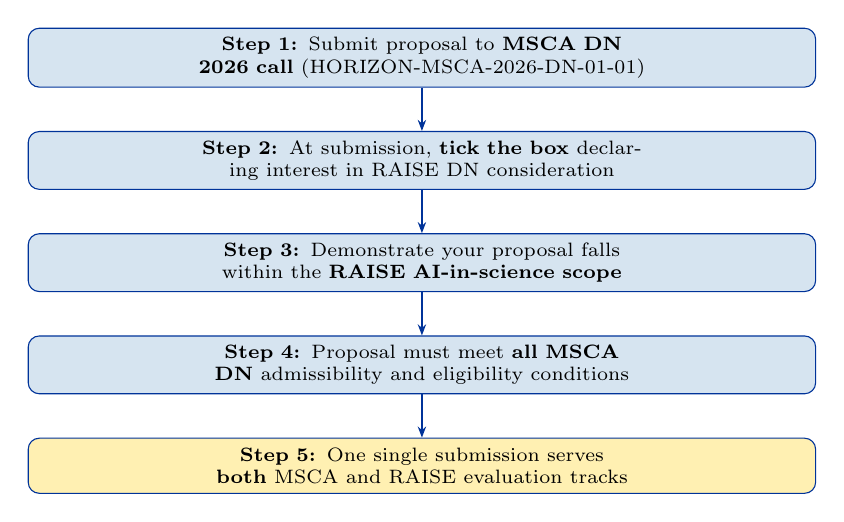
\begin{tikzpicture}[
    node distance=0.55cm,
    every node/.style={font=\scriptsize},
    sbox/.style={draw=euBlue, fill=euLightBlue, rounded corners=4pt,
                 minimum width=10cm, minimum height=0.7cm,
                 text width=9.5cm, align=center},
    arr/.style={-{Stealth[length=4pt]}, euBlue, thick},
  ]
  \node[sbox] (s1)
    {\textbf{Step 1:} Submit proposal to \textbf{MSCA DN 2026 call} (HORIZON-MSCA-2026-DN-01-01)};
  \node[sbox, below=of s1] (s2)
    {\textbf{Step 2:} At submission, \textbf{tick the box} declaring interest in RAISE DN consideration};
  \node[sbox, below=of s2] (s3)
    {\textbf{Step 3:} Demonstrate your proposal falls within the \textbf{RAISE AI-in-science scope}};
  \node[sbox, below=of s3] (s4)
    {\textbf{Step 4:} Proposal must meet \textbf{all MSCA DN} admissibility and eligibility conditions};
  \node[sbox, fill=euGold!30, below=of s4] (s5)
    {\textbf{Step 5:} One single submission serves \textbf{both} MSCA and RAISE evaluation tracks};
  \draw[arr] (s1) -- (s2);
  \draw[arr] (s2) -- (s3);
  \draw[arr] (s3) -- (s4);
  \draw[arr] (s4) -- (s5);
\end{tikzpicture}
\end{center}
\end{frame}

%%% ---------------------------------------------------------------
%%% SLIDE 11 -- EVALUATION OVERVIEW -- TikZ #3
%%% ---------------------------------------------------------------
\begin{frame}{Evaluation Process Overview}
\begin{center}
% -- TikZ Diagram 3: Three-Step Evaluation Pipeline --
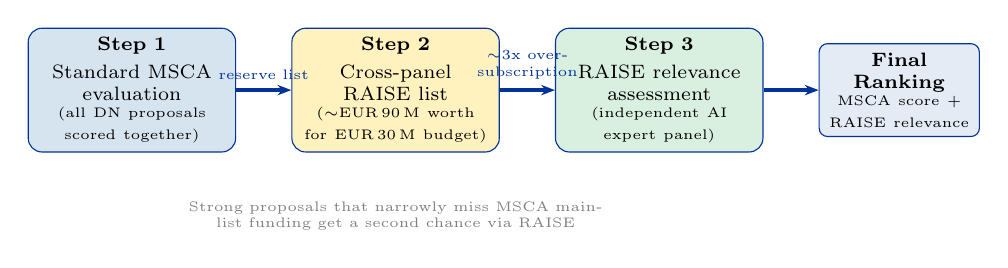
\begin{tikzpicture}[
    every node/.style={font=\scriptsize},
    phase/.style={draw=euBlue, rounded corners=5pt, minimum width=2.6cm,
                  minimum height=1.5cm, text width=2.4cm, align=center,
                  font=\scriptsize},
    arr/.style={-{Stealth[length=5pt]}, euBlue, very thick},
  ]
  % Phase boxes
  \node[phase, fill=euLightBlue] (p1)
    {\textbf{Step 1}\\[2pt]Standard MSCA\\evaluation\\{\tiny(all DN proposals\\scored together)}};
  \node[phase, fill=euGold!25, right=0.7cm of p1] (p2)
    {\textbf{Step 2}\\[2pt]Cross-panel\\RAISE list\\{\tiny(${\sim}$EUR\,90\,M worth\\for EUR\,30\,M budget)}};
  \node[phase, fill=euGreen!15, right=0.7cm of p2] (p3)
    {\textbf{Step 3}\\[2pt]RAISE relevance\\assessment\\{\tiny(independent AI\\expert panel)}};

  % Result box
  \node[draw=euBlue, fill=euBlue!10, rounded corners=3pt,
        minimum width=2cm, minimum height=1.0cm,
        text width=1.8cm, align=center, font=\scriptsize, right=0.7cm of p3]
    (res) {\textbf{Final Ranking}\\{\tiny MSCA score +\\RAISE relevance}};

  % Arrows
  \draw[arr] (p1) -- (p2) node[midway, above, font=\tiny, text=euBlue] {reserve list};
  \draw[arr] (p2) -- (p3) node[midway, above, font=\tiny, text=euBlue, text width=1.4cm, align=center] {${\sim}$3x over-subscription};
  \draw[arr] (p3) -- (res);

  % Annotation
  \node[below=0.5cm of p2, text width=8cm, align=center, font=\tiny, text=gray]
    {Strong proposals that narrowly miss MSCA main-list funding get a second chance via RAISE};
\end{tikzpicture}
\end{center}
\end{frame}

%%% ---------------------------------------------------------------
%%% SLIDE 12 -- MSCA EVALUATION CRITERIA
%%% ---------------------------------------------------------------
\begin{frame}{MSCA Evaluation Criteria}
\renewcommand{\arraystretch}{1.35}
\begin{center}
\begin{tabular}{@{}l c c@{}}
  \toprule
  \textbf{Criterion} & \textbf{Weight} & \textbf{Max Score} \\
  \midrule
  \rowcolor{euLightBlue}
  Excellence        & 50\% & 5.0 \\
  Impact            & 30\% & 5.0 \\
  \rowcolor{euLightBlue}
  Implementation    & 20\% & 5.0 \\
  \bottomrule
\end{tabular}
\end{center}
\vspace{6pt}
\begin{block}{Thresholds and Scoring Rules}
\begin{itemize}
  \item Scoring scale: \textbf{0 to 5}, resolved to \highlight{one decimal place}
  \item Individual criterion threshold: \highlight{3.0 out of 5.0}
  \item Overall funding threshold: \textbf{70\%} (i.e., weighted score $\geq$ 3.5/5.0)
  \item Proposals below \emph{any} threshold are not funded
\end{itemize}
\end{block}
\end{frame}

%%% ---------------------------------------------------------------
%%% SLIDE 13 -- EXCELLENCE (50%)
%%% ---------------------------------------------------------------
\begin{frame}{Excellence (50\%) -- What Evaluators Look For}
\begin{enumerate}
  \item \highlight{Quality and pertinence of R\&I objectives}\\
        {\small Ambitious goals that go beyond the state of the art}
  \item \highlight{Soundness of methodology}\\
        {\small Interdisciplinary approach, gender dimension, open-science practices}
  \item \highlight{Quality and credibility of training programme}\\
        {\small Transferable skills, inter-/multidisciplinary, inter-sectoral components}
  \item \highlight{Quality of supervision}\\
        {\small Mandatory joint supervision for Industrial and Joint Doctorates}
\end{enumerate}
\vspace{6pt}
\textcolor{euBlue}{\small This is the most heavily weighted criterion -- invest the most proposal effort here.}
\end{frame}

%%% ---------------------------------------------------------------
%%% SLIDE 14 -- IMPACT + IMPLEMENTATION
%%% ---------------------------------------------------------------
\begin{frame}{Impact (30\%) + Implementation (20\%)}
\begin{columns}[T]
\begin{column}{0.48\textwidth}
\textbf{\textcolor{euBlue}{Impact (30\%)}}
\begin{itemize}
  \item Contribution to structuring doctoral training at \textbf{European level}
  \item Career perspectives, \textbf{employability}, skills development
  \item Dissemination, exploitation, and communication measures
  \item Magnitude of \textbf{scientific, societal, and economic} impacts
\end{itemize}
\end{column}
\begin{column}{0.48\textwidth}
\textbf{\textcolor{euBlue}{Implementation (20\%)}}
\begin{itemize}
  \item Quality and effectiveness of \textbf{work plan}
  \item Risk assessment and appropriateness of effort per work package
  \item Capacity and \textbf{role of each participant}, hosting arrangements
  \item Consortium bringing \textbf{necessary expertise}
\end{itemize}
\end{column}
\end{columns}
\end{frame}

%%% ---------------------------------------------------------------
%%% SLIDE 15 -- 8 EVALUATION PANELS + TIE-BREAKING
%%% ---------------------------------------------------------------
\begin{frame}{Eight Evaluation Panels}
\begin{columns}[T]
\begin{column}{0.45\textwidth}
\renewcommand{\arraystretch}{1.2}
\begin{tabular}{@{}c l@{}}
  \toprule
  \textbf{Code} & \textbf{Panel} \\
  \midrule
  CHE & Chemistry \\
  \rowcolor{euLightBlue}
  SOC & Social Sciences \& Humanities \\
  ECO & Economic Sciences \\
  \rowcolor{euLightBlue}
  ENG & Information Sci.\ \& Engineering \\
  ENV & Environment \& Geosciences \\
  \rowcolor{euLightBlue}
  LIF & Life Sciences \\
  MAT & Mathematics \\
  \rowcolor{euLightBlue}
  PHY & Physics \\
  \bottomrule
\end{tabular}
\end{column}
\begin{column}{0.50\textwidth}
\textbf{Budget allocation:}\\
Distributed proportionally to eligible proposals per panel.

\vspace{8pt}
\textbf{Tie-breaking order:}
\begin{enumerate}
  \item Excellence score
  \item Impact score
  \item Gender balance of supervisors
  \item Other factors (Green Charter, SME participation, geographical diversity)
\end{enumerate}
\end{column}
\end{columns}
\end{frame}

%%% ---------------------------------------------------------------
%%% SLIDE 16 -- SUCCESS RATES AND COMPETITION
%%% ---------------------------------------------------------------
\begin{frame}{Success Rates and Competition}
\textbf{MSCA DN 2025 data} (most recent round):
\begin{itemize}
  \item 1,616 proposals submitted, 141 funded
  \item Overall success rate: \highlight{8.8\%} (down from 10.5\% in 2024, 12.0\% in 2023)
  \item Average cut-off score: \highlight{94.9\%}
  \item Range: 89.8\% (Economics) to 97.8\% (Environment)
\end{itemize}
\vspace{6pt}
\begin{columns}[T]
\begin{column}{0.48\textwidth}
\begin{exampleblock}{RAISE Advantage}
Adds a \textbf{second funding chance} for strong AI-in-science proposals that narrowly miss the MSCA main list.
\end{exampleblock}
\end{column}
\begin{column}{0.48\textwidth}
\begin{alertblock}{Resubmission Rule}
Proposals scoring \textbf{below 80\%} cannot be resubmitted the following year.\\ {\small ($\geq$70\% of same recruiting organisations triggers resubmission check.)}
\end{alertblock}
\end{column}
\end{columns}
\end{frame}

%%% ---------------------------------------------------------------
%%% SLIDE 17 -- FUNDING PER RESEARCHER (v3 CORRECTED)
%%% ---------------------------------------------------------------
\begin{frame}{Funding Per Researcher (v3 Corrected)}
\renewcommand{\arraystretch}{1.25}
\begin{center}
\small
\begin{tabular}{@{}l r p{5cm}@{}}
  \toprule
  \textbf{Component} & \textbf{EUR/month} & \textbf{Note} \\
  \midrule
  Living allowance        & 4,250 & Adjusted by country correction coeff.\ (CCC) \\
  Mobility allowance      & 710   & Fixed \\
  Family allowance        & 660   & If applicable \\
  \rowcolor{euLightBlue}
  \textbf{Researcher subtotal} & \textbf{5,620} & \textit{Maximum with family} \\
  \midrule
  Research, training, networking & 1,600 & Paid to institution \\
  Management \& indirect         & 1,200 & Paid to institution \\
  \rowcolor{euLightBlue}
  \textbf{Institutional subtotal} & \textbf{2,800} & \\
  \midrule
  \rowcolor{euGold!25}
  \textbf{TOTAL per researcher/month} & \textbf{${\sim}$8,420} & \textit{Max with family} \\
  \bottomrule
\end{tabular}
\end{center}
\vspace{4pt}
\textcolor{euBlue}{\small Employment contract mandatory.  Fellowship option: living allowance \textbf{halved}.}
\end{frame}

%%% ---------------------------------------------------------------
%%% SLIDE 18 -- COUNTRY CORRECTION COEFFICIENTS
%%% ---------------------------------------------------------------
\begin{frame}{Country Correction Coefficients (Examples)}
\renewcommand{\arraystretch}{1.15}
\begin{columns}[T]
\begin{column}{0.50\textwidth}
\footnotesize
\begin{tabular}{@{}l r@{\quad}l r@{}}
  \toprule
  \multicolumn{2}{c}{\textbf{Higher CCC}} & \multicolumn{2}{c}{\textbf{Lower CCC}} \\
  \midrule
  Switzerland & 163.7\% & Poland    & 77.5\% \\
  UK          & 143.5\% & Bulgaria  & 70.0\% \\
  Ireland     & 135.8\% & Romania   & 72.6\% \\
  Denmark     & 131.3\% & Turkey    & 70.0\% \\
  \midrule
  \multicolumn{2}{c}{\textbf{Mid-range}} & \multicolumn{2}{c}{} \\
  \midrule
  France      & 116.6\% & Germany   & 101.5\% \\
  Netherlands & 111.8\% & Belgium   & 100.0\% \\
  \bottomrule
\end{tabular}
\end{column}
\begin{column}{0.46\textwidth}
\textbf{How it works:}\\[4pt]
CCC adjusts the \eur{4,250} living allowance to local cost of living.
\vspace{8pt}

\textbf{Example calculations:}
\begin{itemize}
  \item \textbf{Germany:}\\
        \eur{4,250} $\times$ 101.5\%\\= \highlight{\eur{4,313.75}}/month
  \item \textbf{Denmark:}\\
        \eur{4,250} $\times$ 131.3\%\\= \highlight{\eur{5,580.25}}/month
\end{itemize}
\end{column}
\end{columns}
\end{frame}

%%% ---------------------------------------------------------------
%%% SLIDE 19 -- KEY DATES TIMELINE -- TikZ #4
%%% ---------------------------------------------------------------
\begin{frame}{Key Dates Timeline}
\begin{center}
% -- TikZ Diagram 4: Horizontal Timeline --
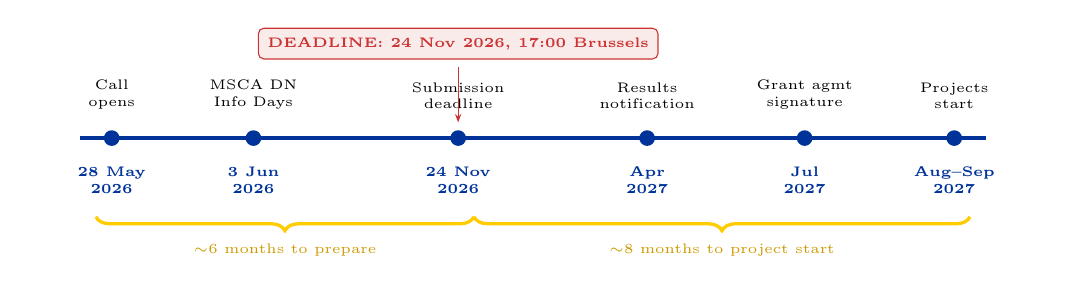
\begin{tikzpicture}[
    every node/.style={font=\scriptsize},
    milestone/.style={circle, fill=euBlue, inner sep=2pt},
    label above/.style={above=7pt, align=center, text width=1.9cm, font=\tiny},
    label below/.style={below=7pt, align=center, font=\tiny\bfseries, text=euBlue},
  ]
  % Timeline axis
  \draw[euBlue, very thick] (0,0) -- (11.5,0);

  % Milestones (explicit to avoid node-name issues)
  \node[milestone] (mA) at (0.4,0) {};
  \node[label above] at (0.4,0) {Call\\opens};
  \node[label below] at (0.4,0) {28 May\\2026};

  \node[milestone] (mB) at (2.2,0) {};
  \node[label above] at (2.2,0) {MSCA DN\\Info Days};
  \node[label below] at (2.2,0) {3 Jun\\2026};

  \node[milestone] (mC) at (4.8,0) {};
  \node[label above] at (4.8,0) {Submission\\deadline};
  \node[label below] at (4.8,0) {24 Nov\\2026};

  \node[milestone] (mD) at (7.2,0) {};
  \node[label above] at (7.2,0) {Results\\notification};
  \node[label below] at (7.2,0) {Apr\\2027};

  \node[milestone] (mE) at (9.2,0) {};
  \node[label above] at (9.2,0) {Grant agmt\\signature};
  \node[label below] at (9.2,0) {Jul\\2027};

  \node[milestone] (mF) at (11.1,0) {};
  \node[label above] at (11.1,0) {Projects\\start};
  \node[label below] at (11.1,0) {Aug--Sep\\2027};

  % Phase annotations
  \draw[euGold, very thick, decorate, decoration={brace, amplitude=5pt, mirror}]
    (0.2,-1.0) -- (5.0,-1.0)
    node[midway, below=6pt, font=\tiny, text=euDarkGold] {${\sim}$6 months to prepare};
  \draw[euGold, very thick, decorate, decoration={brace, amplitude=5pt, mirror}]
    (5.0,-1.0) -- (11.3,-1.0)
    node[midway, below=6pt, font=\tiny, text=euDarkGold] {${\sim}$8 months to project start};

  % Deadline highlight
  \node[draw=euRed, fill=euRed!10, rounded corners=2pt, font=\tiny\bfseries,
        text=euRed] at (4.8,1.2)
    {DEADLINE: 24 Nov 2026, 17:00 Brussels};
  \draw[-{Stealth[length=3pt]}, euRed] (4.8,0.9) -- (4.8,0.2);
\end{tikzpicture}
\end{center}
\end{frame}

%%% ---------------------------------------------------------------
%%% SLIDE 20 -- TIPS FOR A STRONG PROPOSAL
%%% ---------------------------------------------------------------
\begin{frame}{Tips for a Strong RAISE DN Proposal}
\begin{enumerate}
  \item \highlight{Excellence:} Frame AI as the \textbf{central methodology}, not an auxiliary tool; show how it advances the state of the art in the scientific domain
  \item \highlight{AI scope:} Make the \textbf{integral vs.\ instrumental} distinction crystal clear in your proposal text
  \item \highlight{Impact:} Articulate how the network structures doctoral training at \textbf{European level}; include non-academic partners for employability
  \item \highlight{Implementation:} Demonstrate clear work packages with AI development \textbf{delineated}; show consortium expertise balance
  \item \highlight{Supervision:} Plan \textbf{joint supervision} arrangements (mandatory for Industrial and Joint Doctorate types)
  \item \highlight{RAISE relevance:} Explicitly connect \textbf{every} doctoral project to the RAISE AI-in-science definition
\end{enumerate}
\end{frame}

\end{document}
